\documentclass[a4paper,openany,nomultitoc]{dndbook}

\usepackage[british]{babel}

\usepackage[utf8]{inputenc}
\usepackage[singlelinecheck=false]{caption}
\usepackage{lipsum}
\usepackage{listings}
\usepackage{shortvrb}
\usepackage{stfloats}

\captionsetup[table]{labelformat=empty,font={sf,sc,bf,},skip=0pt}

\MakeShortVerb{|}

\usepackage{textgreek}
\usepackage{newunicodechar}
\newunicodechar{π}{\ifmmode\pi\else\textpi\fi}

\lstset{%
  basicstyle=\ttfamily,
  language=[LaTeX]{TeX},
  breaklines=true,
}

\usepackage[hidelinks]{hyperref}

\usepackage{float}

\usepackage{placeins}

\setcounter{tocdepth}{1}

\usepackage{multicol}

\usepackage{tcolorbox}

\usepackage{titling}
\title{The π Tank}
\author{Jamie M Sams}
\date{\today}

\begin{document}
\DndSetThemeColor[DmgLavender]

\frontmatter

%\maketitle
\begin{titlepage}
	\vspace*{\fill}
	\centering
	{\Huge \thetitle}\\
	\vspace*{\fill}
	{\large by \theauthor}
\end{titlepage}

%\tableofcontents

\mainmatter%

\FloatBarrier
\chapter{Hardware}
\FloatBarrier
\begin{multicols}{2}

The platform for this project is the Devastator Tank Mobile Robot Platform from DFRobot (\url{https://www.dfrobot.com/product-1477.html}).  It has four `plates': bottom, left, right and top/front.  The side plates are taken up by the tank tracks, but the top and bottom plates have ample slots and holes to mount any other hardware that would be required.

Attached to the bottom plate via standard PCB standoffs will be the brain of the project: a Raspberry Pi SBC.  I will be opting for the Pi Zero model with a USB WiFi module for network connectivity.

\section{The HAT}

Hardware will be attached to the Pi via a custom-made PCB.  This PCB should accomodate the following features:
\begin{description}
\item[Added]Motor driver
\item[Added]Power supply
\item[Added]Power switch
\item[Added]Stop button
\item[TODO]LEDs for eyes
\end{description}

\end{multicols}

\begin{figure}[hb]
	\begin{center}
		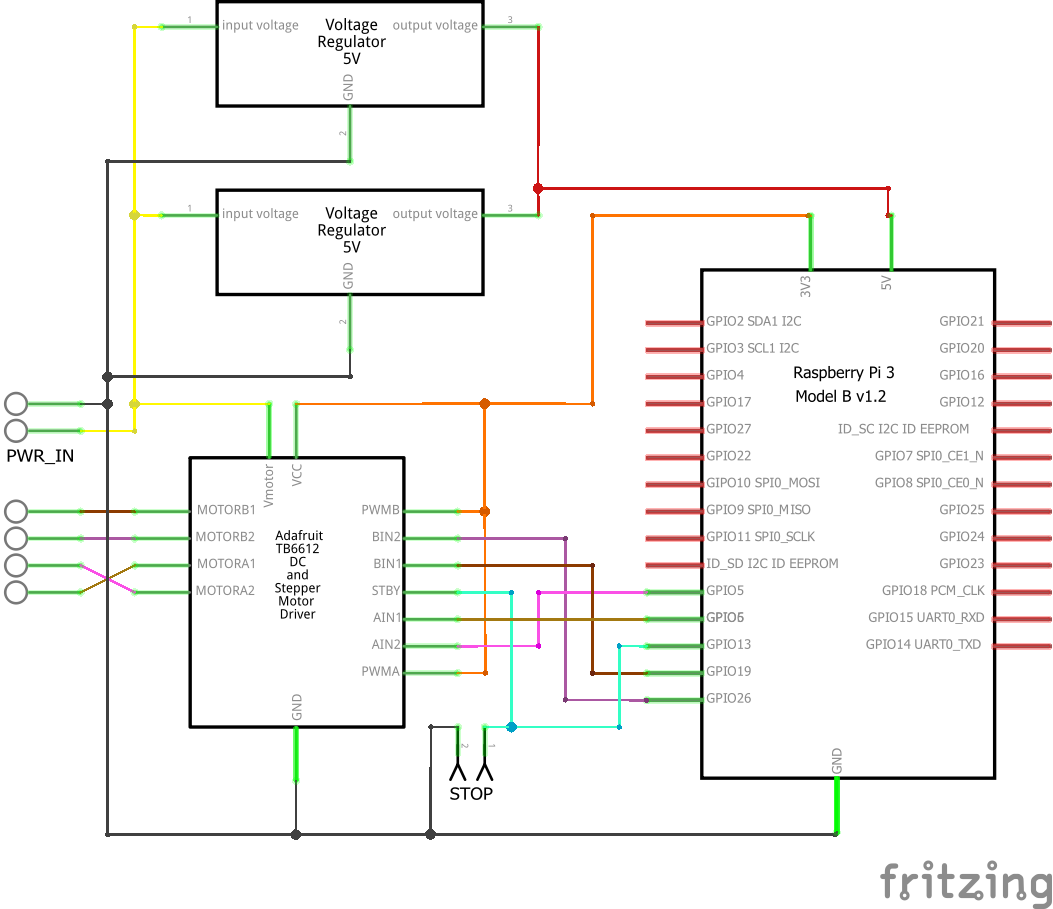
\includegraphics[width=0.95\linewidth]{../PiHat/Pi Hat_schem.png}\\
		{Pi HAT Schematic}
	\end{center}
\end{figure}

\FloatBarrier
\chapter{Software}
\FloatBarrier
\begin{multicols*}{2}

For the OS, the Pi will be running Raspbian Lite.  The control software will be written in Python.

\end{multicols*}

\end{document}